\subsection{PostgreSQL همراه با Pages Huge}
در ابتدا باید به
\lr{PostgreSQL}
بگوییم که از
\lr{huge pages}
استفاده بکند. برای این کار در ابتدا فایل
\linebreak
\codeword{/etc/postgresql/15/main/postgresql.conf}
را باید ادیت کنیم. در این فایل باید اپشن زیر را اضافه کنیم:
\codebox{huge\_pages = on}
سپس باید
\lr{PostgreSQL}
را ری‌استارت کنیم.
سپس با زدن دستور زیر مشاهده می‌کنیم که نتایج عوض شده‌اند:
\codebox{\$ grep $\string^$Huge /proc/meminfo\\
HugePages\_Total:     500\\
HugePages\_Free:      492\\
HugePages\_Rsvd:       64\\
HugePages\_Surp:        0\\
Hugepagesize:       2048 kB\\
Hugetlb:         1024000 kB}
حال دوباره کل تست‌های
\lr{bare metal}
را بر روی
\lr{postgresql}
انجام می‌دهیم.

در حین تست با کرنل  ۴ و ۵ ما شاهد افزایش سرعت حدود ۲۰٪ نسبت به حالت بدون
\lr{huge page}
بودیم. در برخی از مواقع البته شاهد کم شدن سرعت بودیم
(مانند شکل
\ref{fig:postgres:hugepages:kernel6})
ولی در اکثر مواقع سرعت بسیار بالا بود.
اما اتفاق عجیب در کرنل ۶ افتاد. طوری که عملا نمودار
\lr{TPM}
شبیه یک
\lr{ramp}
شده بود. این موضوع به نظر ما یک باگ در کرنل است که می‌تواند بیشتر بررسی در آن صورت بگیرد. چرا که
عملا با اضافه کردن
\lr{huge pages}
به مشکل برخوردیم و در حالت عادی کرنل نسخه‌ی ۶ تفاوت آنچنانی با نسخه‌ی ۵ نداشت.
\begin{figure}[H]
    \centering
    \subfloat{{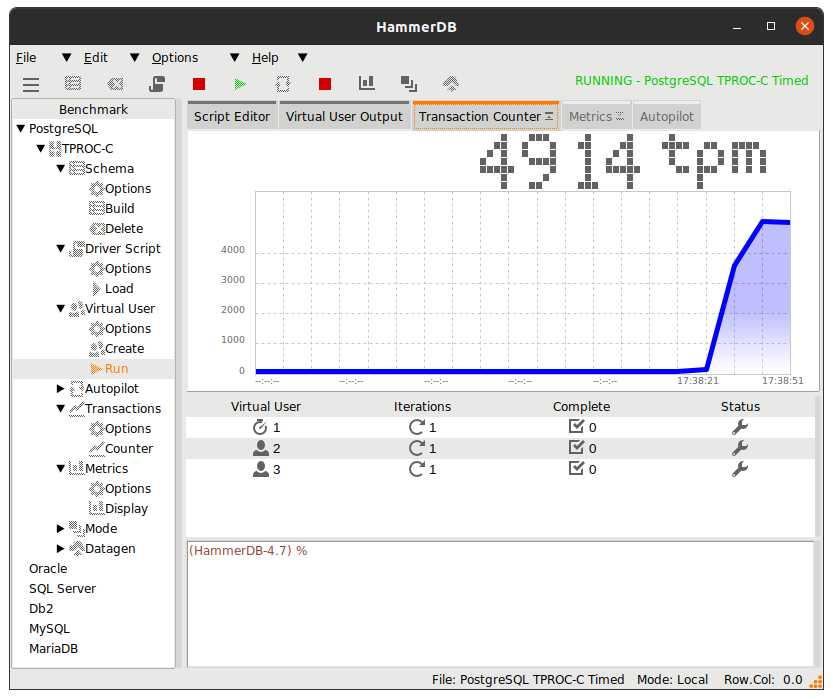
\includegraphics[scale=0.2]{pictures/postgres/huge/huge-5-1.png}}}
    \quad
    \subfloat{{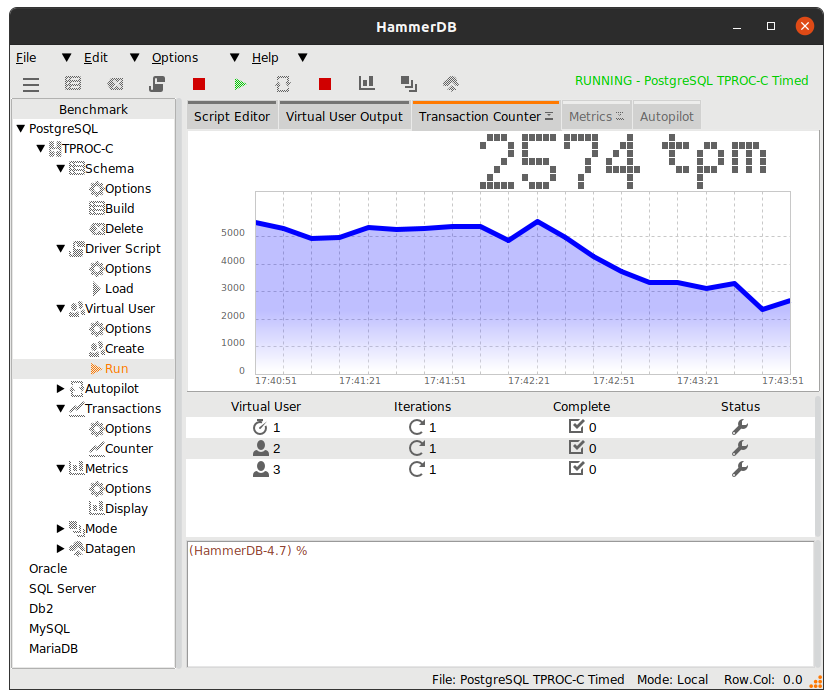
\includegraphics[scale=0.2]{pictures/postgres/huge/huge-5-2.png}}}
    \quad
    \subfloat{{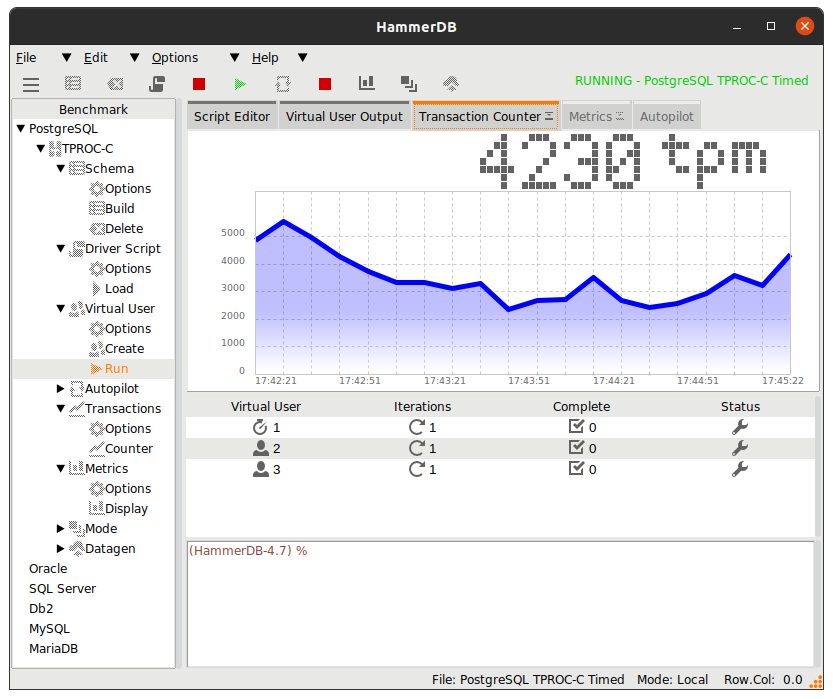
\includegraphics[scale=0.2]{pictures/postgres/huge/huge-5-3.png}}}
    \caption{\lr{TPM} در کرنل ۴ و ۵}
    \label{fig:postgres:hugepages:kernel5}
\end{figure}
\begin{figure}[H]
    \centering
    \subfloat{{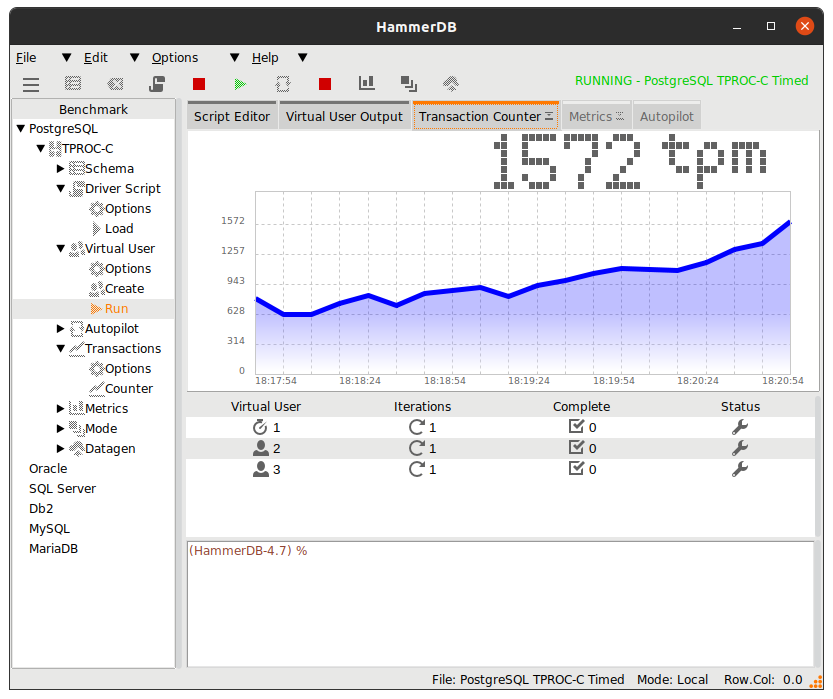
\includegraphics[scale=0.2]{pictures/postgres/huge/huge-6-1.png}}}
    \quad
    \subfloat{{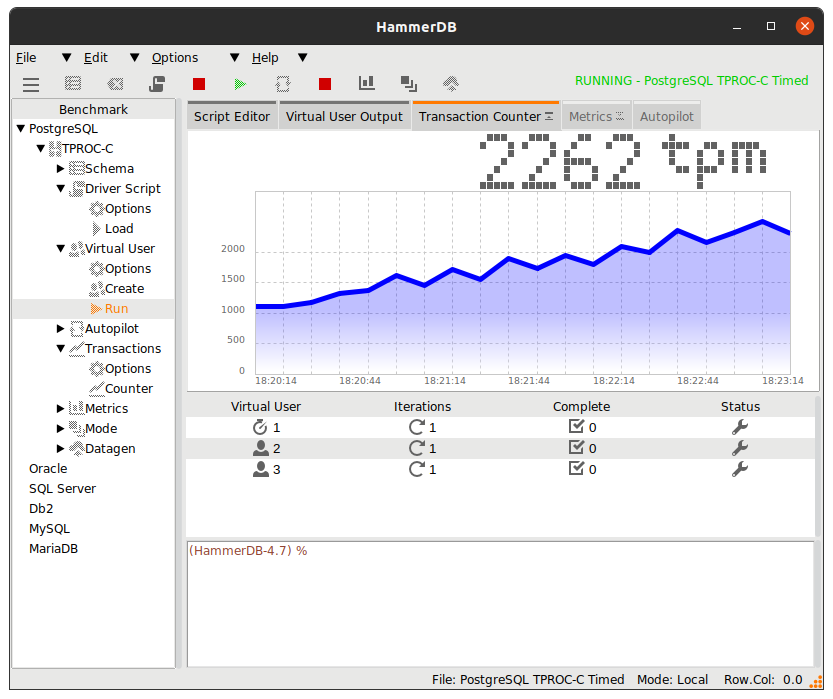
\includegraphics[scale=0.2]{pictures/postgres/huge/huge-6-2.png}}}
    \caption{\lr{TPM} 6}
    \label{fig:postgres:hugepages:kernel6}
\end{figure}